\documentclass[ignorenonframetext,]{beamer}
\setbeamertemplate{caption}[numbered]
\setbeamertemplate{caption label separator}{: }
\setbeamercolor{caption name}{fg=normal text.fg}
\beamertemplatenavigationsymbolsempty
\usepackage{lmodern}
\usepackage{amssymb,amsmath}
\usepackage{ifxetex,ifluatex}
\usepackage{fixltx2e} % provides \textsubscript
\ifnum 0\ifxetex 1\fi\ifluatex 1\fi=0 % if pdftex
  \usepackage[T1]{fontenc}
  \usepackage[utf8]{inputenc}
\else % if luatex or xelatex
  \ifxetex
    \usepackage{mathspec}
  \else
    \usepackage{fontspec}
  \fi
  \defaultfontfeatures{Ligatures=TeX,Scale=MatchLowercase}
\fi
% use upquote if available, for straight quotes in verbatim environments
\IfFileExists{upquote.sty}{\usepackage{upquote}}{}
% use microtype if available
\IfFileExists{microtype.sty}{%
\usepackage{microtype}
\UseMicrotypeSet[protrusion]{basicmath} % disable protrusion for tt fonts
}{}
\newif\ifbibliography
\hypersetup{
            pdftitle={Mesure de la biodiversité et de la structuration spatiale de l'activité économique par l'entropie},
            pdfborder={0 0 0},
            breaklinks=true}
\urlstyle{same}  % don't use monospace font for urls
\usepackage{longtable,booktabs}
\usepackage{caption}
% These lines are needed to make table captions work with longtable:
\makeatletter
\def\fnum@table{\tablename~\thetable}
\makeatother
\usepackage{graphicx,grffile}
\makeatletter
\def\maxwidth{\ifdim\Gin@nat@width>\linewidth\linewidth\else\Gin@nat@width\fi}
\def\maxheight{\ifdim\Gin@nat@height>\textheight0.8\textheight\else\Gin@nat@height\fi}
\makeatother
% Scale images if necessary, so that they will not overflow the page
% margins by default, and it is still possible to overwrite the defaults
% using explicit options in \includegraphics[width, height, ...]{}
\setkeys{Gin}{width=\maxwidth,height=\maxheight,keepaspectratio}

% Prevent slide breaks in the middle of a paragraph:
\widowpenalties 1 10000
\raggedbottom

\AtBeginPart{
  \let\insertpartnumber\relax
  \let\partname\relax
  \frame{\partpage}
}
\AtBeginSection{
  \ifbibliography
  \else
    \let\insertsectionnumber\relax
    \let\sectionname\relax
    \frame{\sectionpage}
  \fi
}
\AtBeginSubsection{
  \let\insertsubsectionnumber\relax
  \let\subsectionname\relax
  \frame{\subsectionpage}
}

\setlength{\parindent}{0pt}
\setlength{\parskip}{6pt plus 2pt minus 1pt}
\setlength{\emergencystretch}{3em}  % prevent overfull lines
\providecommand{\tightlist}{%
  \setlength{\itemsep}{0pt}\setlength{\parskip}{0pt}}
\setcounter{secnumdepth}{0}
\usetheme{PaloAlto}
\usecolortheme{beaver}
\setbeamercolor{section in sidebar}{fg=red!75!green}
\setbeamercolor{section in sidebar shaded}{fg=gray}
\usefonttheme{professionalfonts}

\pgfdeclareimage[width=1.4cm]{logo}{EcoFoG2017.pdf}
\logo{\pgfuseimage{logo}}

% 2-column layout, https://groups.google.com/forum/#!topic/pandoc-discuss/vcy7v9Uk95U
\def\begincols{\begin{columns}}
\def\begincol{\begin{column}}
\def\endcol{\end{column}}
\def\endcols{\end{columns}}

\title{Mesure de la biodiversité et de la structuration spatiale de l'activité
économique par l'entropie}
\date{14 janvier 2018}

\begin{document}
\frame{\titlepage}

\section{Motivation}\label{motivation}

\begin{frame}{La question}

Comment mesurer la structuration spatiale en espace discret?

Applications :

\begin{itemize}
\item
  mesure de la biodiversité ;
\item
  mesure de la concentration spatiale et de la spécialisation en
  économie géographique.
\end{itemize}

\end{frame}

\begin{frame}{Les outils}

L'entropie mesure :

\begin{itemize}
\item
  le désordre (physique statistique, 19\textsuperscript{ème} siècle) ;
\item
  l'incertitude (théorie de l'information, Shannon 1948) ;
\item
  l'inégalité (Theil 1967).
\end{itemize}

\end{frame}

\begin{frame}{La présentation}

Les méthodes utilisées :

\begin{itemize}
\item
  L'entropie classique ;
\item
  Sa généralisation ;
\item
  Les nombres effectifs.
\end{itemize}

Transfert des développement de la littérature sur la biodiversité à
l'économie géographique.

\end{frame}

\section{L'entropie}\label{lentropie}

\begin{frame}{Définir le désordre}

A l'origine, Carnot (\textasciitilde{}1825)

\begin{itemize}
\tightlist
\item
  Second principe de la thermodynamique.
\end{itemize}

Précisément :

\begin{itemize}
\item
  Transfert de chaleur, \(\mathrm{d}Q\), à somme nulle
  (1\textsuperscript{er} principe) ;
\item
  Tiédissement : \(\mathrm{d}Q/T\), à somme positive
  (2\textsuperscript{nd} principe). Augmentation du désordre.
\end{itemize}

Remarque : l'entropie est définie par sa variation (étymologie:
\emph{transformation}).

\end{frame}

\begin{frame}{Boltzmann}

\begincols
 \begincol{.48\textwidth}

Un gaz est un ensemble de particules, chacune ayant plusieurs états
possibles.

L'entropie est proportionnelle au logarithme du nombre d'états possibles
de l'ensemble des particules (1877, traduit par Sharp and Matschinsky
2015).

Lien avec le second principe.

\endcol
 \begincol{.48\textwidth}

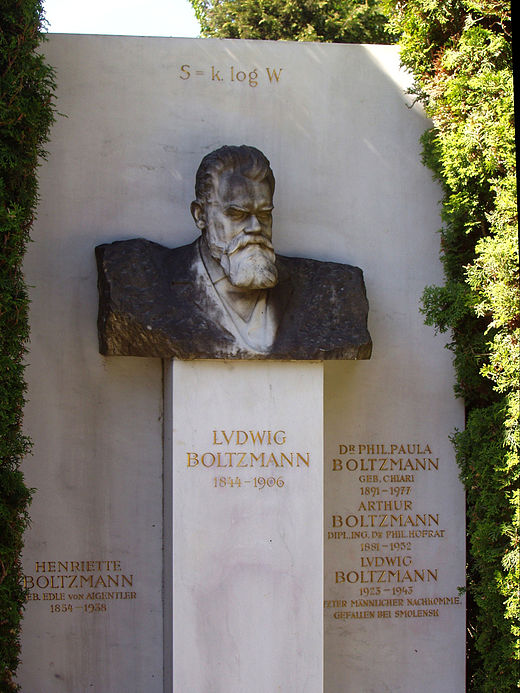
\includegraphics{Images/520px-Zentralfriedhof_Vienna_-_Boltzmann.jpg}

\endcol
\endcols

\end{frame}

\begin{frame}{Mesurer le désordre}

Définition d'une chaîne de caractères :

\begin{itemize}
\item
  longueur \(n\) ;
\item
  alphabet probabilisé.
\end{itemize}

Exemple :

\begin{itemize}
\item
  3 lettres, \{a, b, c\}, fréquences (1/2, 1/3, 1/6) ;
\item
  Combien de chaînes de 60 caractères ?
\item
  Le logarithme du nombre de chaînes est \(n\) fois l'entropie : \(61\).
\end{itemize}

L'entropie de Shannon mesure la complexité de la distribution de \{a, b,
c\}, indépendamment de la longueur de la chaîne : 1.01

\end{frame}

\begin{frame}{Mesurer l'incertitude}

Expérience à plusieurs résultats possibles.

\begin{itemize}
\tightlist
\item
  La probabilité d'obtenir \(r_s\) est \(p_s\).
\end{itemize}

Fonction d'information : \(I(p_s)\), entre \(I(0)=+\infty\) et
\(I(1)=0\).

\begin{itemize}
\item
  Définition : la rareté est \(1/p_s\).
\item
  Le logarithme de la rareté est la fonction d'information de Shannon.
\end{itemize}

L'information apportée par l'ensemble des individus est l'entropie de
Shannon: \[\sum_s{p_s \ln {\frac{1}{p_s}}}\]

\end{frame}

\begin{frame}{Entropie généralisée}

Autres entropies : Rényi, Shorrocks\ldots{} Tsallis (1988)

Paramétriques.

Logarithme déformé :

\includegraphics{Presentation_files/figure-beamer/lnq-1.pdf}

\end{frame}

\begin{frame}{Formalisation}

L'entropie de Tsallis est la moyenne du logarithme (déformé, d'ordre
\(q\)) de la rareté.

L'ordre \(q\) donne une importance plus ou moins grande aux petites
probabilités.

\begin{itemize}
\item
  Entropie d'ordre 0 : le nombre de catégories (-1) ;
\item
  Entropie d'ordre 1 : Shannon ;
\item
  Entropie d'ordre 2 : Simpson (1-Herfindahl).
\end{itemize}

\end{frame}

\begin{frame}{Nombres de Hill}

Nombre de catégories équiprobables de même entropie que celle du système
observé (Hill 1973).

Exponentielle de l'entropie.

Profil de diversité :

\includegraphics[width=0.6\linewidth]{Presentation_files/figure-beamer/Paracou-1}

\end{frame}

\begin{frame}{Entropie relative}

Ecart d'une distribution observée à une distribution attendue.

\begin{itemize}
\item
  Divergence de Kullback-Leibler ;
\item
  Entropie relative de Theil.
\end{itemize}

Généralisation à l'ordre \(q\) (Marcon et al. 2014).

Si la distribution attendue est la moyenne des distributions
(assemblage) alors différence entre l'entropie de l'assemblage et celle
de chaque système.

Transformation en nombres de Hill détaillée plus tard.

\end{frame}

\section{Applications}\label{applications}

\begin{frame}{Questions similaires}

\begincols  \begincol{.65\textwidth}

Biodiversité :

\begin{itemize}
\item
  Nombres d'arbres par espèces dans un habitat forestier : biodiversité.
\item
  Nombres d'arbres par habitat pour une espèce : ubiquité.
\end{itemize}

Economie :

\begin{itemize}
\item
  Nombre d'employés par secteur industriel dans un pays : diversité =
  contraire de la spécialisation.
\item
  Nombre d'employés par pays pour un secteur : ubiquité = contraire de
  la concentration spatiale.
\end{itemize}

\endcol
 \begincol{.35\textwidth}

\emph{Application : 19 industries, 25 pays}.

\begin{longtable}[]{@{}lrr@{}}
\toprule
& AT & BE\tabularnewline
\midrule
\endhead
C10 & 71924 & 85083\tabularnewline
C11 & 9319 & 9814\tabularnewline
C13 & 8665 & 17329\tabularnewline
C14 & 6212 & 3495\tabularnewline
C16 & 32762 & 11271\tabularnewline
C17 & 17078 & 11044\tabularnewline
\bottomrule
\end{longtable}

\endcol
\endcols

\end{frame}

\begin{frame}{Spécialisation absolue}

Transformation simple :

(Maximum possible - Valeur) / (Valeur - 1)

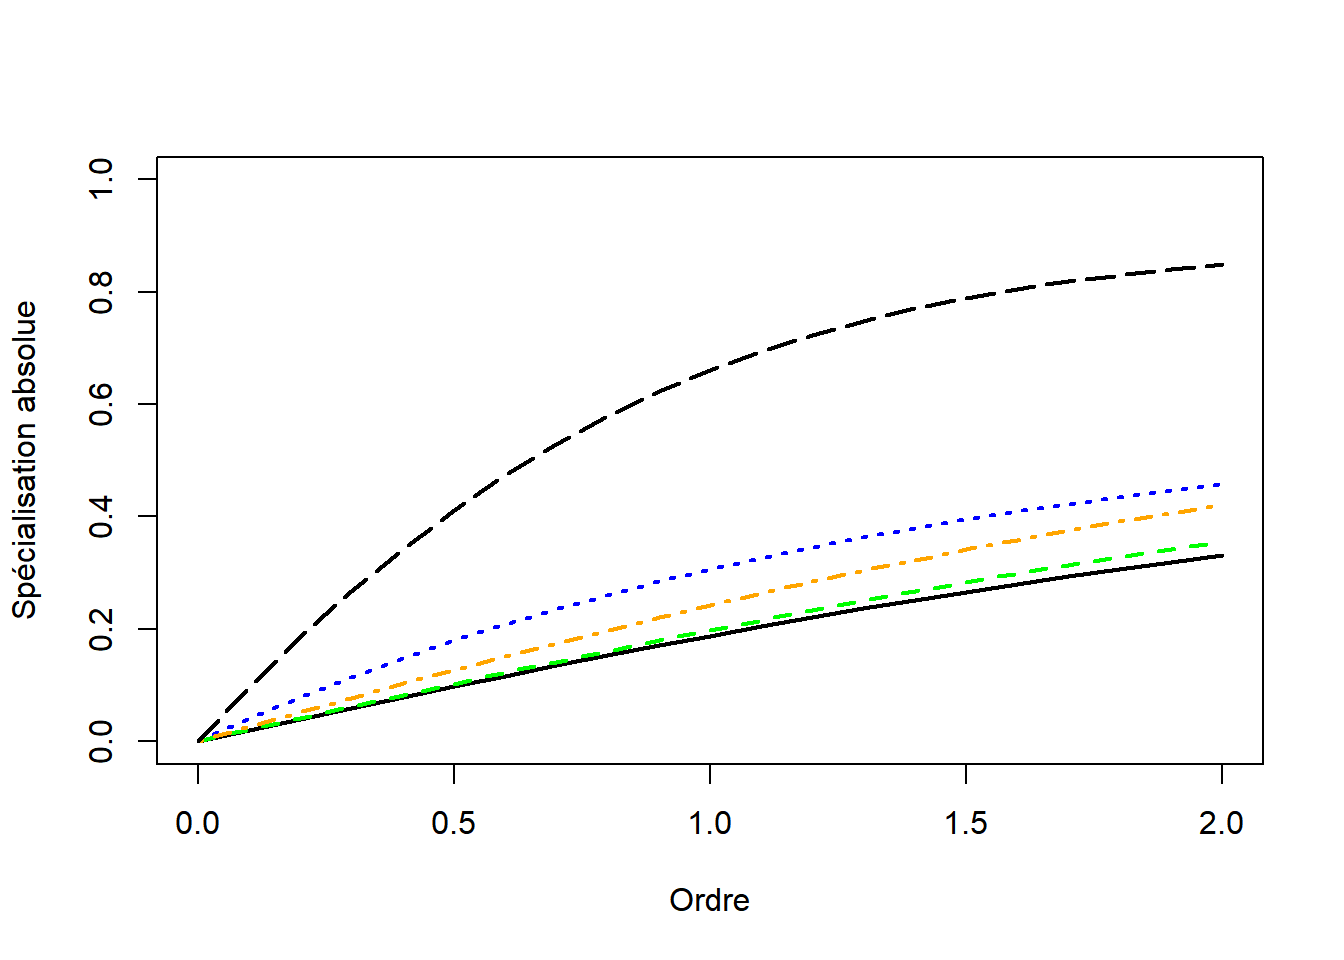
\includegraphics{Presentation_files/figure-beamer/s-1.pdf}

\end{frame}

\begin{frame}{Décomposition de l'entropie}

Exemple : entropie des pays (diversité des secteurs)

\begin{itemize}
\tightlist
\item
  Entropie de l'Europe = moyenne des (entropies absolues + entropies
  relatives des pays).
\end{itemize}

Nombres de Hill :

\begin{itemize}
\tightlist
\item
  Diversité de l'Europe = Diversité moyenne des pays x nombre de pays
  effectifs.
\end{itemize}

Classique en écologie : diversités \(\gamma\), \(\alpha\) et \(\beta\).

\end{frame}

\begin{frame}{Exemple}

Diversité des secteurs industriels en Europe :

\includegraphics{Presentation_files/figure-beamer/de-1.pdf}

\end{frame}

\begin{frame}{Décomposition de la diversité jointe}

Diversité de l'ensemble des effectifs : nombres d'employés par secteur
et par pays.

\begin{itemize}
\tightlist
\item
  Nombre effectif d'unités.
\end{itemize}

Décomposition de l'entropie et de la diversité similaire, un élément
supplémentaire: la redondance (Gregorius 2010).

Diversité jointe = Nombre effectif de secteurs par pays x nombre de pays
effectifs x \emph{redondance des pays}.

\end{frame}

\begin{frame}{Diversité jointe}

Concentration spatiale de l'industrie européenne :

\includegraphics{Presentation_files/figure-beamer/ce-1.pdf}

\end{frame}

\section{Conclusion}\label{conclusion}

\begin{frame}{Concepts identiques, expression contraire}

Diversité \(\leftrightarrow\) Spécialisation.

Ubiquité \(\leftrightarrow\) Concentration.

Raison : mise en avant de l'aspect positif.

\end{frame}

\begin{frame}{Absolu et relatif}

Approches complémentaires dans la littérature économique.

Unification par l'entropie :

\begin{itemize}
\item
  liens étroits : significativité de l'une \(\iff\) significativité de
  l'autre ;
\item
  information très différente.
\end{itemize}

\end{frame}

\begin{frame}{Interfertilisation}

De la physique à l'écologie : entropie de Tsallis.

De la théorie de l'information à l'écologie : divergence de Kullback and
Leibler (1951).

De la théorie de l'information à l'économie : entropie relative de
Theil.

En écologie : nombres effectifs.

En écologie théorique : redondance.

\end{frame}

\begin{frame}{Références}

\tiny

\hypertarget{refs}{}
\hypertarget{ref-Gregorius2010}{}
Gregorius, Hans-Rolf. 2010. ``Linking Diversity and Differentiation.''
\emph{Diversity} 2 (3): 370--94.
doi:\href{https://doi.org/10.3390/d2030370}{10.3390/d2030370}.

\hypertarget{ref-Hill1973}{}
Hill, M. O. 1973. ``Diversity and Evenness: A Unifying Notation and Its
Consequences.'' \emph{Ecology} 54 (2): 427--32.
doi:\href{https://doi.org/10.2307/1934352}{10.2307/1934352}.

\hypertarget{ref-Kullback1951}{}
Kullback, S., and R. A. Leibler. 1951. ``On Information and
Sufficiency.'' \emph{The Annals of Mathematical Statistics} 22 (1):
79--86.

\hypertarget{ref-Marcon2014a}{}
Marcon, Eric, Ivan Scotti, Bruno Hérault, Vivien Rossi, and Gabriel
Lang. 2014. ``Generalization of the Partitioning of Shannon Diversity.''
\emph{Plos One} 9 (3): e90289.
doi:\href{https://doi.org/10.1371/journal.pone.0090289}{10.1371/journal.pone.0090289}.

\hypertarget{ref-Shannon1948}{}
Shannon, Claude E. 1948. ``A Mathematical Theory of Communication.''
\emph{The Bell System Technical Journal} 27: 379--423, 623--56.

\hypertarget{ref-Sharp2015}{}
Sharp, Kim, and Franz Matschinsky. 2015. ``Translation of Ludwig
Boltzmann's paper `on the relationship between the second fundamental
theorem of the mechanical theory of heat and probability calculations
regarding the conditions for thermal equilibrium'.'' \emph{Entropy} 17
(4): 1971--2009.
doi:\href{https://doi.org/10.3390/e17041971}{10.3390/e17041971}.

\hypertarget{ref-Theil1967}{}
Theil, H. 1967. \emph{Economics and Information Theory}. Chicago: Rand
McNally \& Company.

\hypertarget{ref-Tsallis1988}{}
Tsallis, Constantino. 1988. ``Possible generalization of Boltzmann-Gibbs
statistics.'' \emph{Journal of Statistical Physics} 52 (1): 479--87.
doi:\href{https://doi.org/10.1007/BF01016429}{10.1007/BF01016429}.

\end{frame}

\end{document}
